\label{powerlaw}

\section{Power Law Processes}

\frame[t] {
\frametitle{Power Law Distribution}
A power law distribution is a distribution whose tail falls off as
\[ P(X=x) \propto x^{-\alpha} \]
For some $\alpha > 1$.  The simplest such distribution is the zeta distribution on natural numbers:
\[ f_\alpha(k) = \frac{k^{-\alpha}}{\zeta(\alpha)} \]
and the Pareto distribution on the real line (with small-scale cutoff $x_{min} > 0$):
\[ f_\alpha(x) = \frac{\alpha-1}{x_{min}} \left(\frac{x}{x_{min}}\right)^{-\alpha} \]
}

\frame[t] {
\frametitle{Scale Free Property}
A power law distribution on the real line is {\em scale free} in the sense that, for all scales $k > 0$ and $x > x_{min}$
\[  f_{\alpha}(kx) \propto f_{\alpha}(x) \]
Where the proportionality constant depends only on $k$.
}

\frame[t] {
\frametitle{Power Laws in Nature}
Words in natural language, arranged by frequency \cite{Zipf1965}.
\begin{center}
\includegraphics[scale=0.35]{figs/wikipedia-zipf.png} \\
Log-log plot of word frequency in Wikipedia (source: Wikipedia)
\end{center}
}

\frame[t] {
\frametitle{Power Laws in Nature}
Cities arranged by population \cite{Blank2000}.
}

\frame[t] {
\frametitle{Power Laws in Nature}
Earthquakes arranged by magnitude \cite{Gutenberg1955}. \\
\begin{center}
\includegraphics[scale=0.35]{figs/earthquakes.png} \\
(image source: http://quake.usgs.gov/recenteqs/latest.htm)
\end{center}
}

\frame[t] {
\frametitle{Power Laws in Nature}
Power spectra of natural images \cite{Ruderman1994}.
\begin{center}
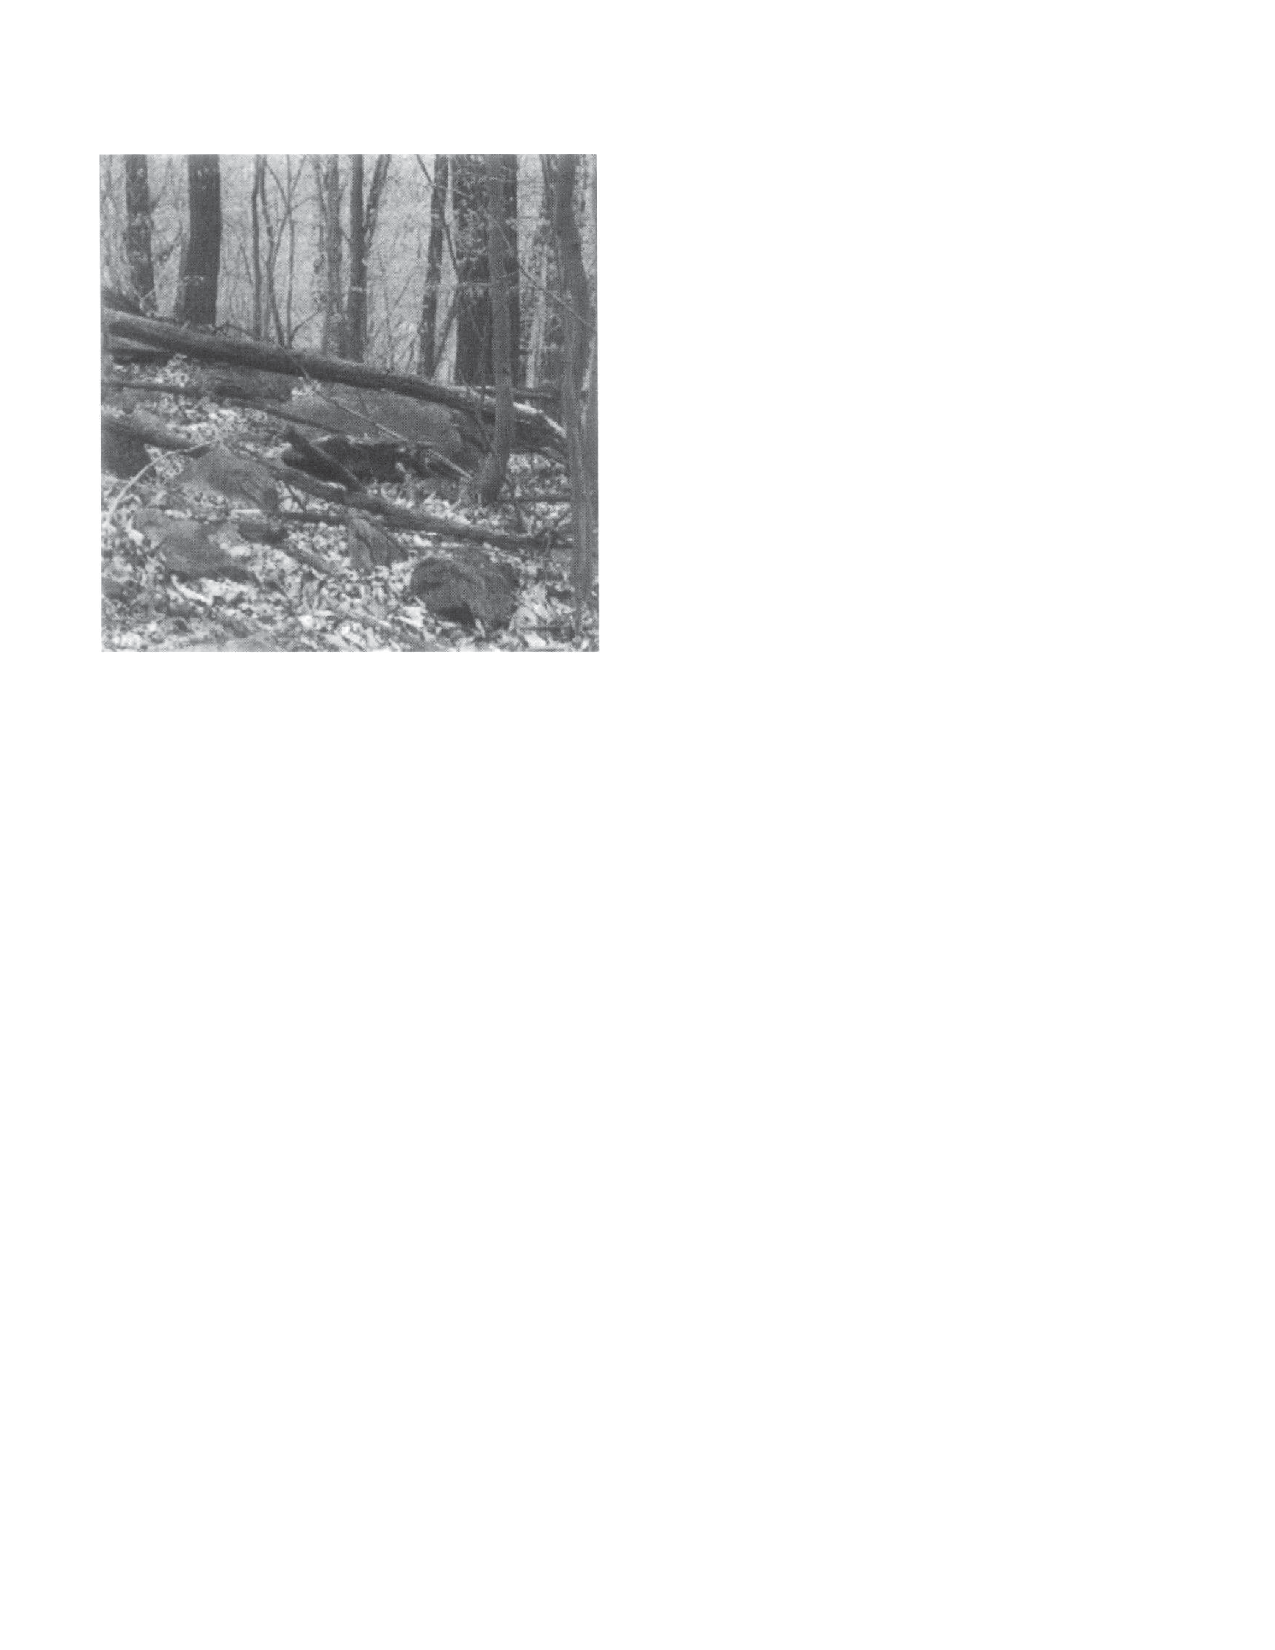
\includegraphics[scale=0.5]{figs/ruderman_bialek_img.pdf}
\hspace*{5 mm}
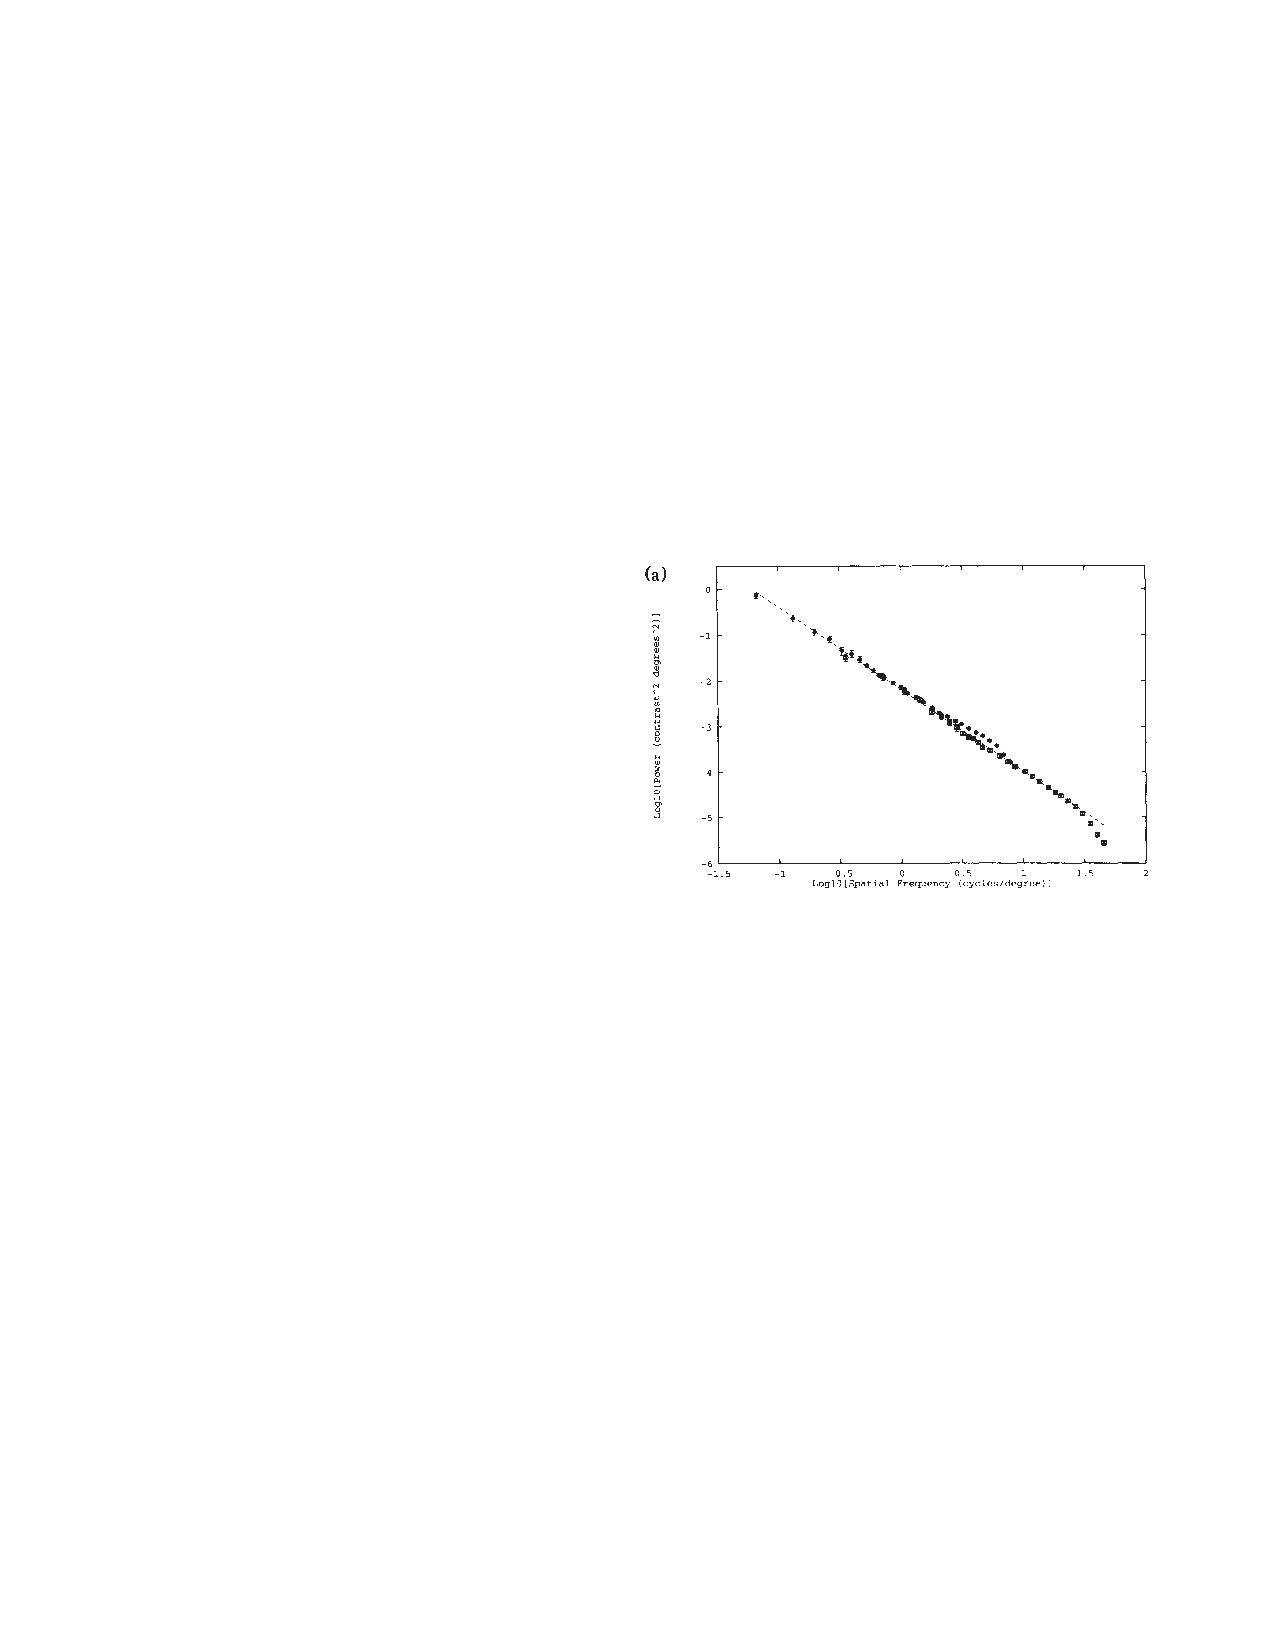
\includegraphics[scale=0.75]{figs/ruderman_bialek_plot.pdf}
\end{center}
}

\frame[t] {
\frametitle{Pitman Yor Process: Definition}
A natural class of distributions for modeling data with power-law clustering is the Pitman-Yor process (PYP).  A Pitman-Yor process $PY(c,d,H)$ is a distribution over distributions with three parameters:
\begin{itemize}
\item A discount $ 0 \le d < 1 $ that controls the length of the tails of the distribution
\item A concentration $c > -d$ that controls the variance of draws from a PYP
\item A base distribution $H$ which is, pointwise, the mean of a draw from a PYP
\end{itemize}
A draw $G \sim PY(c,d,H)$ is atomic: it can be expressed as a countable number of point masses that sum to one: 
\[G = \sum_{k=1}^{\infty} \pi_k \delta_{\phi_k}\].  
}

\frame[t]{
\frametitle{PYP: Stick-Breaking Construction}
A simple generative procedure for $\pi_k$ and $\phi_k$ is given by the stick-breaking construction:
\[
\begin{array}{rcll}
\beta_k  & \sim & Beta(1-d, c+kd) & \forall \, k = 1 \ldots \infty \\
&&& \\
\pi_k & = &  \beta_k \prod_{i=1}^{k-1}(1- \beta_i) & \forall \, k = 1 \ldots \infty \\
&&& \\
\phi_k  & \sim &  H & \forall \, k = 1 \ldots \infty
\end{array}
\]

The expected length of a stick $\mathbb{E}[\pi_k]$ falls off as a power law for large $k$ when $d \ne 0$.  When $d = 0$ the stick lengths fall off exponentially, and the PYP reduces to a Dirichlet process.
%The expected length of a stick is $\mathbb{E}[\pi_k] = \mathbb{E}[\beta_k]\prod_{i=1}^{k-1}(1 - \mathbb{E}[\beta_i]) = \frac{1-d}{1+c+(k-1)d}\prod_{i=1}^{k-1}\frac{c+id}{1+c+(i-1)d} = d(1-d)\frac{\Gamma(\frac{c}{d} + (k-1))}{\Gamma(\frac{c}{d})}\frac{\Gamma(\frac{1+c}{d})}{\Gamma(\frac{1+c}{d} + k)}$
}

\frame[t] {
\frametitle{PYP: Chinese Restaurant Representation}
Due to the atomic nature of $G \sim PY(c,d,H)$, draws from $G$ cluster together.  If we want to know the probability that new data will have the same value as some observed data, we can integrate out $G$ and represent this probability only in terms of $c$, $d$ and the observed data $\theta_{1 \ldots N}$.  Say the data is distributed across $K$ clusters, each with $n_k$ data points, then we have

\begin{eqnarray*}
p(\theta_{N+1} \text{ is in cluster } k | \theta_{1 \ldots N} ) & = & \frac{n_k - d}{c+N} \\
p(\theta_{N+1} \text{ is in a new cluster} | \theta_{1 \ldots N} ) & = & \frac{c + Kd}{c + N}
\end{eqnarray*}

This is the two-parameter {\em Chinese Restaurant Process}.  As the discount introduces a bias against sitting at an occupied table, the distribution of table sizes is heavy-tailed.

}